% !TEX TS-program = pdflatex
% !TEX root = ../ArsClassica.tex

%************************************************
\chapter{CPLEX}

\label{chp:3-CPLEX}

%************************************************
\section{Plain Execution}
We simply create the linear programming model and then we pass it to \textsc{CPLEX} for the optimization. The performances, as we will notice for all the methods, depend on the instance. We noticed the power of \textsc{CPLEX} which finds the optimal solution in few seconds, and in the meantime we discovered that some instances take many hours to be solved by our machines. 
The main steps of our code in this phase are: 
\begin{itemize}
\item Read the input files and the command line parameter and parse them;
\item Memorize turbines and cables;
\item Develop the specific linear programming model;
\item Call CPX\_INT\_OPT that optimizes the instance;
\item Ask to \textsc{CPLEX} the optimal function;
\item Print and graph it;
\end{itemize}

\subsection{Relaxed Mode}
Sometimes there are constraints that risk to block the improvement of the solution or make \textsc{CPLEX} take longer before finding a feasible solution. \\
To avoid those situations, it is possible to \textit{"relax"} some constraints in order to speed up the process of searching for the first solution. The main steps are to add a slack variable $\geq 0$ in the model and then add this variable in the objective function multiplied for a constant reasonably large. In this way, even if \textsc{CPLEX} could find a wrong initial solution, it is probable that this solution will rapidly improve and be corrected. Anyway, the choice to relax some constraint should not affect the optimal solution because of the very high impact on the objective function. \\
In our case we found three constraints that could be relaxed: the maximum number $C$ of edges entering in a substation, the flux losses and the need to have one big connected component that connects all the arcs (for some heuristic algorithm). \\
The first constraint can be relaxed in this way (see the result in image \ref{img:relax1}):
\[
f^{R_1}_{obj} (x,y,k) = f_{obj} (x,y,k) + BIG\_M\_CABLE \cdot s
\]
\[
c \geq \sum^n_{i=1} y_{ih} -s \quad \forall \ h : P_h = -1
\]
The second constraint, about the flux losses, can be relaxed in this way (see the result in image \ref{img:relax2}):
\[
f^{R_2}_{obj} (x,y,k) = f_{obj} (x,y,k) + BIG\_M\_CABLE \cdot \sum^n_{i=1} s_i
\]
\[
\sum^n_{i=1} f_{hs} = \sum^n_{i=1} f_{ih} + P_h - s_h \quad \forall h = 1, ... n
\]
And finally it is possible to add to the relaxed constraint $f^{R_2}_{obj} (x,y,k)$ also the third option, simply adding the following constraint (see the result in image \ref{img:relax3}): 
\[
\sum^n_{j=1} y_{ij} < 1 \quad \forall i = 1, ... n
\]
We listed the three different possibility that we can activate in our algorithms. The second and the third options come out of thinking about heuristic algorithm, while the first option can be applied in all the algorithms. 
\begin{center}
	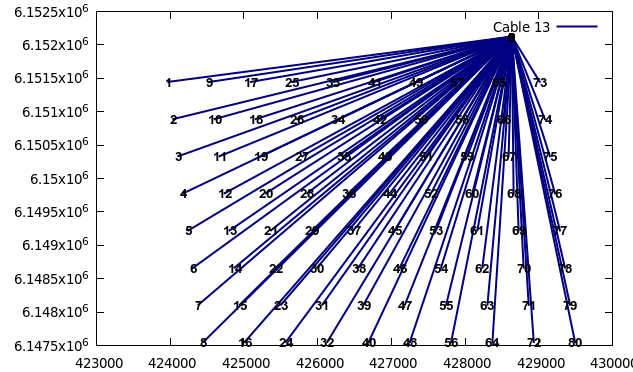
\includegraphics[scale=0.4]{Graphics/data02-relax1.png}
	\captionof{figure}{Example relax 1}
	\label{img:relax1}
\end{center}

\begin{center}
	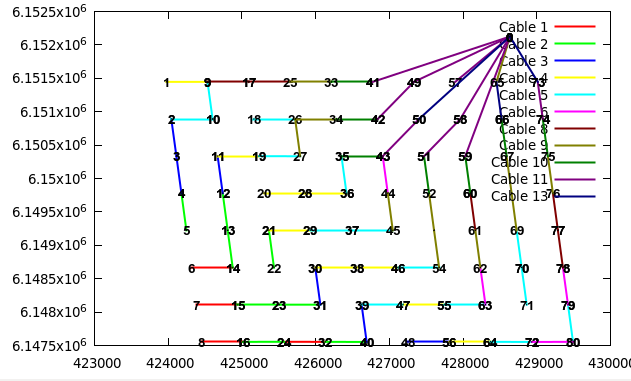
\includegraphics[scale=0.4]{Graphics/data02-relax2.png}
	\captionof{figure}{Example relax 2}
	\label{img:relax2}
\end{center}

\begin{center}
	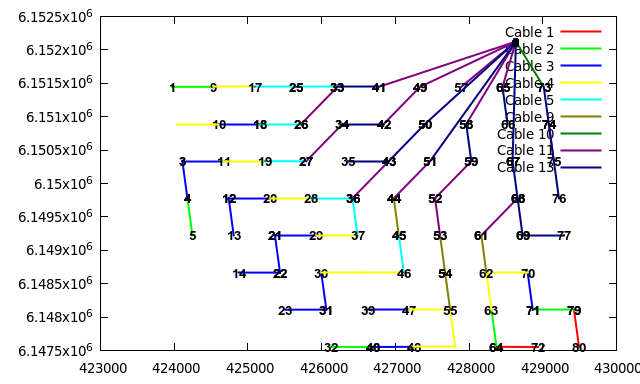
\includegraphics[scale=0.4]{Graphics/data02-relax3.png}
	\captionof{figure}{Example relax 3}
	\label{img:relax3}
\end{center}
\subsection{CPLEX Heuristics-Params}
The \textsc{CPLEX} code contains some heuristic procedures. Being integrated into branch \& cut, they can speed the final proof of optimality or provide a suboptimal but high-quality solution in a shorter amount of time than by branching alone. With default parameter settings, \textsc{CPLEX} automatically invokes the heuristics when they seem likely to be beneficial. However, it is possible to adapt them to our specific case and instances by changing the frequency of activation of these procedures by setting some \textsc{CPLEX} parameter. We mainly analyzed two of them:
\begin{itemize}
\setlength{\parskip}{0pt}
\setlength{\itemsep}{0pt plus 1pt}
\item \textbf{RINS}: it means \textit{Relaxation induced neighborhood search} and it is a heuristic that explores a neighborhood of the current incumbent solution to try to find a new, improved incumbent. In the initial part the process does not change, but as soon as a solution is found the RINS heuristic tries to improve it with more frequency. It is possible to infer that the RINS method has been used in a \textsc{CPLEX} step when in the logs there is a ‘*’ near to the number. We set the \textit{-rins} param to 5 in all the tests. 
\item \textbf{POLISHING}: this heuristic tries to modify some variables of a (good) solution to improve it. It is possible to set a condition that enables this method, in order to avoid premature usage of this method, which that can lead to wasted time and performances. We decided not to change this parameter in our tests.
\end{itemize}

\section{Lazy Constraints Method}
The generated constraints are often too much and risk to block the solution for a long time if we added to the model statically.  
Instead of adding systematically all the constraints in the model at the beginning, we generate them "on the fly" when they are violated by the Branch and Bound process. In this way \textsc{CPLEX} will check those constraints only when a solution is created. In the case that some constraint is violated, \textsc{CPLEX} will add the corresponding constraint before the incumbent update. \\
The \textsc{CPLEX} command to add a set of constraints is \textit{CPXAddLazyConstraints}. \\
This technique decreases the efficiency of the \textsc{CPLEX} pre-processing and sometimes the computation time of the solution is really high, but generally gives good results.

\section{Loop Method}
In this method the \textsc{CPLEX} execution will be reiterated until the optimal solution is not found. From this feature comes his name. \\
The model that we initially use do not include the no-crossing constraints and it is not possible to set all of them at one time. So in this method, we add time by time only the necessary constraints after each loop of the method. In particular after each loop we must verify that the chosen cables do not intersect.\\
This method is mathematically correct, but seems inefficient. However, nowadays the power of \textsc{CPLEX} pre-processing allows the Loop Method to be considered. We have also implemented a variant of this method that can stop the execution in some cases, even if the optimality has not yet been reached. This optimization comes from the fact that often \textsc{CPLEX} spends a lot of time demonstrating the optimality of a solution. However, maybe this solution uses some crossing cables. The stopping conditions can be several: stop at the first solution (not so good in our case because often it is the "star solution"), stop when the gap is less than a fixed percentual or stop after a timelimit. \\
In our solution we chose a variant of the timelimit condition. We have defined \textit{timestart} and \textit{timeloop} parameters: when the algorithm starts \textsc{CPLEX} runs for \textit{timestart} seconds searching for a good starting solution, then the loops will last \textit{timeloop} seconds, until the real \textit{timelimit} expires. The main reason of this choice is to seek for a good solution before the starting of the real Loop method. \\ 
This technique solves consecutively more complex models. It is important to note that, if no new constraint is added to the model, \textsc{CPLEX} can restart from the last solution found saving a lot of time. One limitation of this method is that at the end it is possible (especially in the case of few loops iterations) to have crossing edges because initially the \textsc{CPLEX} solver is launched without constraints. 
\section{Lazy Callback Method}
\textsc{CPLEX} supports callbacks so that it is possible to define functions that will be called at crucial points in the application. In particular, lazy constraints are constraints that the user knows are unlikely to be violated, and in consequence, the user
wants them applied lazily, not before needed. Lazy constraints are only (and always) checked when an integer feasible solution candidate has been identified, and any of these constraints that is violated will be applied to the full model. \\
In this method we have added the no-crossing constraint calling the \textit{lazy constraint callback} (named "LazyConstraintCallBack") each time the solver find an integer feasible solution. \\
The algorithm starts with the creation of the model, and the lazy constraint callback is installed to make \textsc{CPLEX} call it when needed. Then, the \textsc{CPLEX} solver starts to resolve the model applying the branch-and-cut technique. When \textsc{CPLEX} finds an integer feasible solution, the lazy constraint callback is called. The solution that we have now is an integer solution of the problem where, perhaps, some of
the arcs intersects. Hence, starting from this solution we have to check if there are cables crossing and, if there are any, we have to add the corresponding constraints. In this way, only necessary constraints are added and \textsc{CPLEX} will make sure that these constraints will be satisfied before producing any future solution of the problem.\\
The algorithm terminates when \textsc{CPLEX} finds the optimal integer solution without crossing, or when the \textit{timelimit} is reached. \\
Different from the loop method, \textsc{CPLEX} generates the optimal solution only for the final model, adding the constraints during the resolution of the problem. This tendentially leads to the addition of more constraints in respect to the loop method, hence in some cases, leading to a slower execution.

\section{Results}
With the objective to compare our algorithms we have executed various instances
of the Wind Farm Cable Problem analyzing their solution after five and ten minutes for each method. All the instances have 30, 80 or 100 turbines with the number of cables that varying by 3 to 13 types. In this table we can see the result of this execution. As we can see the first method, the basic method with \textsc{CPLEX} that contains also all the cross constraints does not work bad but it initially has a lot of problem to compute the model because sometimes we have too many constraints, in some case our computers are blocked ( in the table: nan). To escape from this problem we set the no cross constraints as lazy constraint using the pool of lazy constraints of \textsc{CPLEX}, the lazy callback and the loop method. As we can see there are not more differences between the first two method, nothing that can be attributed to one method considering the performance variability. Also if we consider the mean of gaps between the solution with the \textsc{CPLEX} pool and the lazy callbacks, the method with \textsc{CPLEX} pool has the best results in ten minutes while in five minutes win the method with lazy callbacks. The method to compute the gap that we used is:
\[gap = \frac{(solution 1 - solution 2)}{(solution 1 + solution 2)}\] with solution 1 and 2 relative to the same instance.The sign of the gap tell us which the method wins.\\
While the loop method seems to be the worst method and have a problem, the loop method must be start from a good solution before than it iterate and removes the cross, so we have, as first, compute a solution with half of time of the total execution of method. \\ 

\begin{table}[!h]
\caption{\textsc{CPLEX} based methods results with \textit{timelimit} 5 minutes}
\begin{tabular}{lllllllll}
\hline
Instance & \multicolumn{2}{l}{\textbf{CPX basic}} & \multicolumn{2}{l}{\textbf{CPX lazy const}} & \multicolumn{2}{l}{\textbf{CPX loop (60s)}} & \multicolumn{2}{l}{\textbf{CPX lazy callback}} \\ \hline
         & time                & solution                & time                  & solution                 & time               & solution               & time                 & solution                \\ \hline
data\_01 & 300                 & 2.45E+07                & 300                   & 2.05E+07                 & 300                & 2.13E+07               & 300                  & 1.98E+07                \\
data\_02 & nan                 & nan                     & 300                   & 2.16E+07                 & 300                & 2.45E+07               & 300                  & 4.02E+09                \\
data\_03 & 300                 & 2.58E+07                & 300                   & 7.02E+09                 & 300                & 2.35E+07               & 300                  & 2.35E+07                \\
data\_04 & 301                 & 3.14E+07                & 300                   & 2.48E+07                 & 300                & 2.66E+07               & 300                  & 2.48E+07                \\
data\_05 & 300                 & 1.00E+08                & 300                   & 7.02E+09                 & 300                & 7.00E+10               & 300                  & 2.40E+07                \\
data\_06 & nan                 & nan                     & 300                   & 4.02E+09                 & 300                & 3.49E+07               & 300                  & 3.02E+09                \\
data\_07 & 3                   & 8.56E+06                & 4                     & 8.56E+06                 & 4                  & 8.56E+06               & 300                  & 8.66E+06                \\
data\_08 & 8                   & 8.81E+06                & 9                     & 8.81E+06                 & 7                  & 8.81E+06               & 192                  & 8.81E+06                \\
data\_09 & 9                   & 1.01E+07                & 31                    & 1.01E+07                 & 2                  & 1.01E+07               & 3                    & 1.01E+07                \\
data\_10 & 6                   & 1.03E+07                & 8                     & 1.03E+07                 & 10                 & 1.03E+07               & 24                   & 1.03E+07                \\
data\_12 & 13                  & 8.60E+06                & 2                     & 8.60E+06                 & 3                  & 8.60E+06               & 300                  & 8.58E+06                \\
data\_13 & 7                   & 8.93E+06                & 5                     & 8.93E+06                 & 4                  & 8.93E+06               & 9                    & 8.93E+06                \\
data\_14 & 16                  & 1.02E+07                & 26                    & 1.02E+07                 & 3                  & 1.02E+07               & 12                   & 1.02E+07                \\
data\_15 & 14                  & 1.03E+07                & 7                     & 1.03E+07                 & 5                  & 1.03E+07               & 34                   & 1.03E+07                \\
data\_16 & 225                 & 8.05E+06                & 20                    & 8.05E+06                 & 21                 & 8.05E+06               & 30                   & 8.05E+06                \\
data\_17 & 88                  & 8.56E+06                & 142                   & 8.56E+06                 & 300                & 8.56E+06               & 300                  & 8.56E+06                \\
data\_18 & 300                 & 8.36E+06                & 140                   & 8.36E+06                 & 300                & 8.36E+06               & 300                  & 8.36E+06                \\
data\_19 & 102                 & 9.18E+06                & 161                   & 9.18E+06                 & 300                & 9.27E+06               & 46                   & 9.21E+06                \\
data\_20 & 300                 & 1.99E+08                & 300                   & 1.20E+10                 & 300                & 4.50E+10               & 300                  & 1.30E+10                \\
data\_21 & 300                 & 1.17E+08                & 300                   & 8.04E+09                 & 300                & 3.10E+10               & 117                  & 1.50E+10                \\
data\_26 & 300                 & 2.34E+07                & 300                   & 7.03E+09                 & 300                & 9.00E+10               & 300                  & 2.29E+07                \\
data\_27 & nan                 & nan                     & 300                   & 2.50E+07                 & 300                & 2.65E+07               & 299                  & 2.39E+07                \\
data\_28 & nan                 & nan                     & 300                   & 1.70E+10                 & 300                & 3.35E+07               & 204                  & 1.20E+10                \\
data\_29 & nan                 & nan                     & 300                   & 4.65E+07                 & 300                & 4.65E+07               & 2                    & 9.30E+10                \\ \hline
\end{tabular}
\end{table}

\begin{table}[!h]
\caption{\textsc{CPLEX} based methods results with \textit{timelimit} 10 minutes}
\begin{tabular}{lllllll}
\hline
Instance & \multicolumn{2}{l}{\textbf{CPX lazy const}} & \multicolumn{2}{l}{\textbf{CPX loop (120 s)}} & \multicolumn{2}{l}{\textbf{CPX laxy callback}} \\ \hline
         & time               & solution               & time                & solution                & time                 & solution                \\ \hline
data\_01 & 600                & 1.95E+07               & 600                 & 2.07E+07                & 600                  & 2.04E+07                \\
data\_02 & 600                & 2.38E+07               & 600                 & 2.15E+07                & 588                  & 2.49E+07                \\
data\_03 & 600                & 2.27E+07               & 480                 & 2.27E+07                & 600                  & 2.27E+07                \\
data\_04 & 600                & 2.45E+07               & 600                 & 2.54E+07                & 600                  & 2.45E+07                \\
data\_05 & 600                & 2.46E+07               & 600                 & 2.46E+07                & 500                  & 2.42E+07                \\
data\_06 & 600                & 2.74E+07               & 480                 & 2.74E+07                & 577                  & 2.74E+07                \\
data\_07 & 3                  & 8.56E+06               & 600                 & 8.56E+06                & 6                    & 8.56E+06                \\
data\_08 & 19                 & 8.81E+06               & 3                   & 8.81E+06                & 45                   & 8.81E+06                \\
data\_09 & 22                 & 1.01E+07               & 3                   & 1.01E+07                & 4                    & 1.01E+07                \\
data\_10 & 12                 & 1.03E+07               & 5                   & 1.03E+07                & 50                   & 1.03E+07                \\
data\_12 & 2                  & 8.60E+06               & 3                   & 8.60E+06                & 1                    & 8.60E+06                \\
data\_13 & 6                  & 8.93E+06               & 4                   & 8.93E+06                & 11                   & 8.93E+06                \\
data\_14 & 4                  & 1.02E+07               & 3                   & 1.02E+07                & 9                    & 1.02E+07                \\
data\_15 & 7                  & 1.03E+07               & 8                   & 1.03E+07                & 37                   & 1.03E+07                \\
data\_16 & 14                 & 8.05E+06               & 22                  & 8.05E+06                & 14                   & 8.05E+06                \\
data\_17 & 149                & 8.56E+06               & 63                  & 8.56E+06                & 67                   & 8.56E+06                \\
data\_18 & 213                & 8.36E+06               & 71                  & 8.36E+06                & 491                  & 8.36E+06                \\
data\_19 & 211                & 9.18E+06               & 26                  & 9.18E+06                & 342                  & 9.18E+06                \\
data\_20 & 600                & 4.01E+07               & 360                 & 4.01E+07                & 110                  & 1.70E+12                \\
data\_21 & 600                & 4.70E+07               & 360                 & 4.70E+07                & 96                   & 1.30E+12                \\
data\_26 & 600                & 2.27E+07               & 480                 & 2.27E+07                & 600                  & 2.28E+07                \\
data\_27 & 600                & 2.42E+07               & 600                 & 2.37E+07                & 600                  & 2.42E+07                \\
data\_28 & 600                & 2.84E+07               & 240                 & 2.84E+07                & 600                  & 2.69E+07                \\
data\_29 & 600                & 3.09E+07               & 600                 & 3.09E+07                & 600                  & 3.00E+12                \\ \hline
\end{tabular}
\end{table}


\begin{center}
	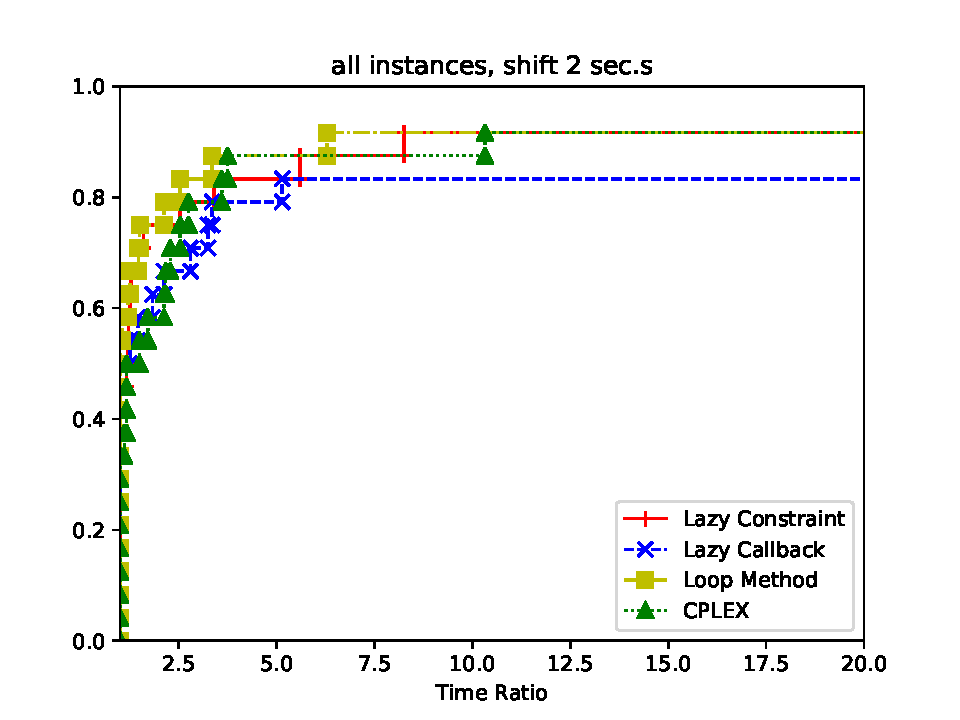
\includegraphics[scale=0.7]{Graphics/cplex5.pdf}
	\captionof{figure}{Performance profile for CPLEX methods with \textit{timelimit} 5 minutes}
	\label{img:mathperfprof}
\end{center}

\begin{center}
	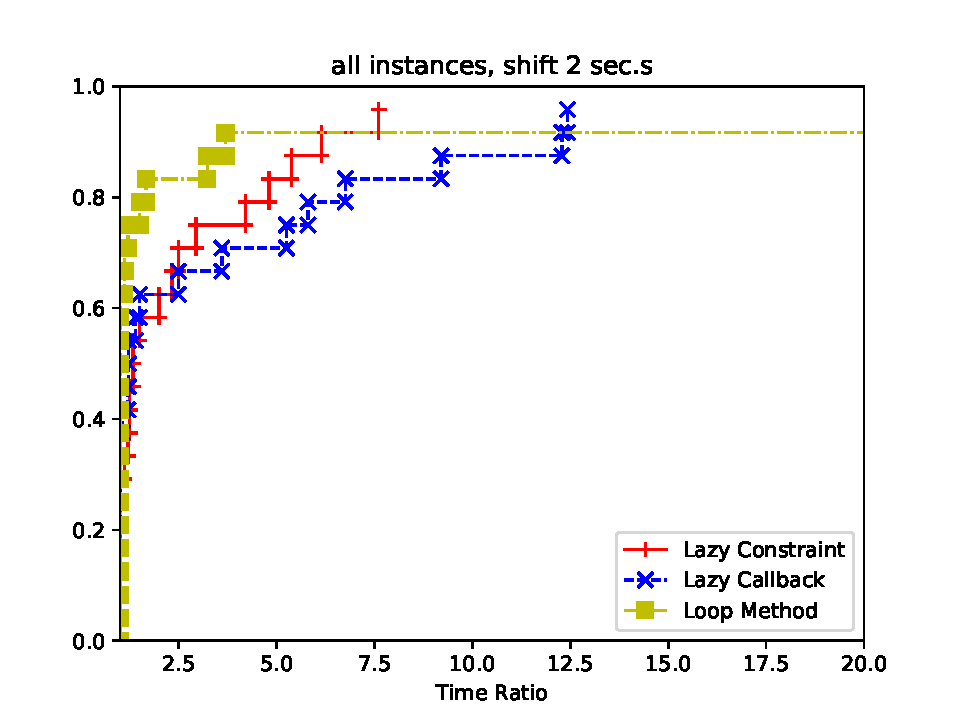
\includegraphics[scale=0.7]{Graphics/cplex.pdf}
	\captionof{figure}{Performance profile for CPLEX methods with \textit{timelimit} 10 minutes}
	\label{img:mathperfprof}
\end{center}